\chapter{排序算法}

\section{排序算法}

\subsection{排序算法}

应用到排序的常见比比皆是,例如当开发一个学生管理系统时需要按照学号从小到大进行排序,当开发一个电商平台时需要把同类商品按价格从低到高进行排序,当开发一款游戏时需要按照游戏得分从多到少进行排序。\\

根据时间复杂度的不同,主流的排序算法可以分为三类:

\begin{enumerate}
	\item $ O(n^2) $:冒泡排序、选择排序、插入排序
	\item $ O(nlogn) $:归并排序、快速排序、堆排序
	\item $ O(n) $:计数排序、桶排序、基数排序
\end{enumerate}

在算法界还存在着更多五花八门的排序,它们有些基于传统排序变形而来,有些则是脑洞大开,如鸡尾酒排序、猴子排序、睡眠排序等。\\

例如睡眠排序,对于待排序数组中的每一个元素,都开启一个线程,元素值是多少,就让线程睡多少毫秒。当这些线程陆续醒来的时候,睡得少的线程线性来,睡得多的线程后醒来。睡眠排序虽然挺有意思,但是没有任何实际价值。启动大量线程的资源消耗姑且不说,数值接近的元素也未必能按顺序输出,而且一旦遇到很大的元素,线程睡眠时间可能超过一个月。\\

\subsection{稳定性}

排序算法还可以根据其稳定性,划分为稳定排序和不稳定排序:

\begin{itemize}
	\item 稳定排序:值相同的元素在排序后仍然保持着排序前的顺序。
	\item 不稳定排序:值相同的元素在排序后打乱了排序前的顺序。
\end{itemize}

\begin{figure}[H]
	\centering
	\begin{tikzpicture}[font=\ttfamily,
			array/.style={matrix of nodes,nodes={draw, minimum size=10mm, fill=green!30},column sep=-\pgflinewidth, row sep=0.5mm, nodes in empty cells,
					row 1/.style={nodes={draw=none, fill=none, minimum size=5mm}},
				}]

		\draw (-4,0.7) node{原始数列};
		\draw (-3.8,-0.3) node{不稳定排序};
		\draw (-4,-1.4) node{稳定排序};

		\matrix[array] (array) {
			0 & 1 & 2                     & 3                     & 4 \\
			5 & 8 & \textcolor{orange}{6} & \textcolor{purple}{6} & 3 \\
			3 & 5 & \textcolor{purple}{6} & \textcolor{orange}{6} & 8 \\
			3 & 5 & \textcolor{orange}{6} & \textcolor{purple}{6} & 8 \\
		};
	\end{tikzpicture}
	\caption{排序稳定性}
\end{figure}

\newpage

\section{冒泡排序}

\subsection{冒泡排序(Bubble Sort)}

冒泡排序是最基础的交换排序。冒泡排序之所以叫冒泡排序,正是因为这种排序算法的每一个元素都可以像小气泡一样,根据自身大小,一点一点向着数组的一侧移动。\\

按照冒泡排序的思想,要把相邻的元素两两比较,当一个元素大于右侧相邻元素时,交换它们的位置;当一个元素小于或等于右侧相邻元素时,位置不变。\\

例如一个有8个数字组成的无序序列,进行升序排序。

\begin{figure}[H]
	\centering
	\begin{tikzpicture}[font=\ttfamily,
			array/.style={matrix of nodes,nodes={draw, minimum size=10mm, fill=green!30},column sep=-\pgflinewidth, row sep=0.5mm, nodes in empty cells,
					row 1/.style={nodes={draw=none, fill=none, minimum size=5mm}},
				}]

		\matrix[array] (array) {
			0 & 1 & 2 & 3 & 4 & 5 & 6 & 7 \\
			5 & 8 & 6 & 3 & 9 & 2 & 1 & 7 \\
			5 & 8 & 6 & 3 & 9 & 2 & 1 & 7 \\
			5 & 6 & 8 & 3 & 9 & 2 & 1 & 7 \\
			5 & 6 & 3 & 8 & 9 & 2 & 1 & 7 \\
			5 & 6 & 3 & 8 & 9 & 2 & 1 & 7 \\
			5 & 6 & 3 & 8 & 2 & 9 & 1 & 7 \\
			5 & 6 & 3 & 8 & 2 & 1 & 9 & 7 \\
			5 & 6 & 3 & 8 & 2 & 1 & 7 & 9 \\
		};

		\draw[-, very thick, red] (-4,3.95) rectangle (-2,2.95);
		\draw[-, very thick, red] (-3,2.85) rectangle (-1,1.89);
		\draw[-, very thick, red] (-2,1.8) rectangle (0,0.79);
		\draw[-, very thick, red] (-1,0.71) rectangle (1,-0.25);
		\draw[-, very thick, red] (0,-0.35) rectangle (2,-1.33);
		\draw[-, very thick, red] (1,-1.39) rectangle (3,-2.4);
		\draw[-, very thick, red] (2,-2.49) rectangle (4,-3.47);

		\draw[<->, very thick, red] (-2.4,2.4) -- (-1.6,2.4);
		\draw[<->, very thick, red] (-1.35,1.3) -- (-0.6,1.3);
		\draw[<->, very thick, red] (0.6,-0.8) -- (1.4,-0.8);
		\draw[<->, very thick, red] (1.65,-1.9) -- (2.4,-1.9);
		\draw[<->, very thick, red] (2.65,-2.95) -- (3.4,-2.95);

		\draw[-, very thick, blue] (3,-3.55) rectangle (4,-4.55);
	\end{tikzpicture}
	\caption{冒泡排序第1轮}
\end{figure}

这样一来,元素9作为数列中最大的元素,就像是汽水里的小气泡一样,浮到了最右侧。这时,冒泡排序的第1轮就结束了。数列最右侧元素9的位置可以认为是一个有序区域,有序区域目前只有1个元素。\\

接着进行第2轮排序:

\begin{figure}[H]
	\centering
	\begin{tikzpicture}[font=\ttfamily,
			array/.style={matrix of nodes,nodes={draw, minimum size=10mm, fill=green!30},column sep=-\pgflinewidth, row sep=0.5mm, nodes in empty cells,
					row 1/.style={nodes={draw=none, fill=none, minimum size=5mm}},
				}]

		\matrix[array] (array) {
			0 & 1 & 2 & 3 & 4 & 5 & 6 & 7 \\
			5 & 6 & 3 & 8 & 2 & 1 & 7 & 9 \\
			5 & 6 & 3 & 8 & 2 & 1 & 7 & 9 \\
			5 & 3 & 6 & 8 & 2 & 1 & 7 & 9 \\
			5 & 3 & 6 & 8 & 2 & 1 & 7 & 9 \\
			5 & 3 & 6 & 2 & 8 & 1 & 7 & 9 \\
			5 & 3 & 6 & 2 & 1 & 8 & 7 & 9 \\
			5 & 3 & 6 & 2 & 1 & 7 & 8 & 9 \\
		};

		\draw[-, very thick, red] (-4,3.4) rectangle (-2,2.4);
		\draw[-, very thick, red] (-3,2.3) rectangle (-1,1.37);
		\draw[-, very thick, red] (-2,1.27) rectangle (0,0.29);
		\draw[-, very thick, red] (-1,0.2) rectangle (1,-0.77);
		\draw[-, very thick, red] (0,-0.86) rectangle (2,-1.84);
		\draw[-, very thick, red] (1,-1.92) rectangle (3,-2.9);

		\draw[<->, very thick, red] (-2.4,1.85) -- (-1.6,1.85);
		\draw[<->, very thick, red] (-0.4,-0.3) -- (0.4,-0.3);
		\draw[<->, very thick, red] (0.6,-1.35) -- (1.4,-1.35);
		\draw[<->, very thick, red] (1.6,-2.4) -- (2.4,-2.4);

		\draw[-, very thick, blue] (3,3.4) rectangle (4,2.4);
		\draw[-, very thick, blue] (3,2.32) rectangle (4,1.33);
		\draw[-, very thick, blue] (3,1.25) rectangle (4,0.26);
		\draw[-, very thick, blue] (3,0.2) rectangle (4,-0.8);
		\draw[-, very thick, blue] (3,-0.9) rectangle (4,-1.85);
		\draw[-, very thick, blue] (3,-1.95) rectangle (4,-2.9);
		\draw[-, very thick, blue] (2,-3) rectangle (4,-4);
	\end{tikzpicture}
	\caption{冒泡排序第2轮}
\end{figure}

第2轮排序结束后,数列右侧的有序区有了2个元素。\\

根据相同的方法,完成剩下的排序:

\begin{figure}[H]
	\centering
	\begin{tikzpicture}[font=\ttfamily,
			array/.style={matrix of nodes,nodes={draw, minimum size=10mm, fill=green!30},column sep=-\pgflinewidth, row sep=0.5mm, nodes in empty cells,
					row 1/.style={nodes={draw=none, fill=none, minimum size=5mm}},
				}]

		\matrix[array] (array) {
			0 & 1 & 2 & 3 & 4 & 5 & 6 & 7 \\
			3 & 5 & 2 & 1 & 6 & 7 & 8 & 9 \\
			3 & 2 & 1 & 5 & 6 & 7 & 8 & 9 \\
			2 & 1 & 3 & 5 & 6 & 7 & 8 & 9 \\
			1 & 2 & 3 & 5 & 6 & 7 & 8 & 9 \\
			1 & 2 & 3 & 5 & 6 & 7 & 8 & 9 \\
		};

		\draw (-5,1.9) node{第3轮};
		\draw (-5,0.8) node{第4轮};
		\draw (-5,-0.3) node{第5轮};
		\draw (-5,-1.4) node{第6轮};
		\draw (-5,-2.4) node{第7轮};

		\draw[-, very thick, blue] (1,2.32) rectangle (4,1.33);
		\draw[-, very thick, blue] (0,1.25) rectangle (4,0.26);
		\draw[-, very thick, blue] (-1,0.2) rectangle (4,-0.8);
		\draw[-, very thick, blue] (-2,-0.9) rectangle (4,-1.85);
		\draw[-, very thick, blue] (-3,-1.95) rectangle (4,-2.9);
	\end{tikzpicture}
	\caption{冒泡排序第3 $ \sim $ 7轮}
\end{figure}

\vspace{0.5cm}

\subsection{算法分析}

冒泡排序是一种稳定排序,值相等的元素并不会打乱原本的顺序。由于该排序算法的每一轮都要遍历所有元素,总共遍历n - 1轮。

\begin{table}[H]
	\centering
	\setlength{\tabcolsep}{5mm}{
		\begin{tabular}{|c|c|c|c|}
			\hline
			\textbf{时间复杂度} & \textbf{空间复杂度} & \textbf{稳定性} & \textbf{设计思想} \\
			\hline
			$ O(n^2) $          & $ O(1) $            & 稳定            & 贪心法            \\
			\hline
		\end{tabular}
	}
	\caption{冒泡排序算法分析}
\end{table}

\mybox{冒泡排序}

\begin{lstlisting}[language=C]
void bubbleSort(int *arr, int n) {
    for(int i = 0; i < n; i++) {
        for(int j = 0; j < n-i-1; j++) {
            if(arr[j] > arr[j+1]) {
                swap(&arr[j], &arr[j+1]);
            }
        }
    }
}
\end{lstlisting}

\vspace{0.5cm}

\mybox{逆序对}\\

假设数组有n个元素,如果A[i] > A[j], i < j,那么A[i]和A[j]就被称为逆序对(inversion)。

\begin{lstlisting}[language=C]
int countInversions(int *arr, int n) {
    int cnt = 0;        // 逆序对数
    for(int i = 0; i < n-1; i++) {
        for(int j = i+1; j < n; j++) {
            if(arr[i] > arr[j]) {
                cnt++;
            }
        }
    }
    return cnt;
}
\end{lstlisting}

\vspace{0.5cm}

\subsection{冒泡排序第一次优化}

常规的冒泡排序需要进行n - 1轮循环,即使在中途数组已经有序,但是还是会继续剩下的循环。例如当数组是\{2, 1, 3, 4, 5\}时,在经过一轮排序后已经变为有序状态,再进行多余的循环就会浪费时间。\\

为了解决这个问题,可以在每一轮循环中设置一个标志。如果该轮循环中有元素发生过交换,那么就有必要进行下一轮循环。如果没有发生过交换,说明当前数组已经完成排序。\\

\mybox{冒泡排序第一次优化}

\begin{lstlisting}[language=C]
void bubbleSortOptimize1(int *arr, int n) {
    for(int i = 0; i < n - 1; i++) {
        bool hasSwapped = false;  // 标记是否发生交换
        for(int j = 0; j < n - i - 1; j++) {
            if(arr[j] > arr[j+1]) {
                swap(&arr[j], &arr[j+1]);
                hasSwapped = true;    // 发生交换
            }
        }
        // 该轮未发生交换,已经有序
        if(!hasSwapped) {
            return;
        }
    }
}
\end{lstlisting}

\vspace{0.5cm}

\subsection{冒泡排序第二次优化}

在经过一次优化后,算法还存在一个问题,例如数组\{2, 3, 1, 4, 5, 6\}在经过一轮交换后变为\{2, 1, 3, 4, 5, 6\},但是在下一轮时后面有很多次比较都是多余的,因为并没有产生交换操作。\\

为了解决这个问题,可以再设置一个标志位,用于记录当前轮所交换的最后一个元素的下标。在下一轮排序中,只需比较到该标志位即可,因此之后的元素在上一轮中没有交换过,在这一轮中也不可能交换了。\\

\mybox{冒泡排序第二次优化}

\begin{lstlisting}[language=C]
void bubbleSortOptimize2(int *arr, int n) {
    int len = n - 1;        // 内层循环执行次数
    for(int i = 0; i < n - 1; i++) {
        bool hasSwapped = false;  // 标记是否发生交换
        int last = 0;       // 标记最后一次发生交换的位置
        for(int j = 0; j < len; j++) {
            if(arr[j] > arr[j+1]) {
                swap(&arr[j], &arr[j+1]);
                hasSwapped = true;    // 发生交换
                last = j;
            }
        }
        // 该轮未发生交换,已经有序
        if(!hasSwapped) {
            return;
        }
        len = last;         // 最后一次发生交换的位置
    }
}
\end{lstlisting}

\newpage

\section{选择排序}

\subsection{选择排序(Selection Sort)}

有了冒泡排序为什么还要发明选择排序?冒泡排序有个很大的弊端,就是元素交换次数太多了。\\

想象一个场景,假设你是一名体育老师,正在指挥一群小学生按照个头从矮到高的顺序排队。采用冒泡排序的方法需要频繁交换相邻学生的位置,同学们心里恐怕会想:“这体育老师是不是有毛病啊?”\\

在程序运行的世界里,虽然计算机并不会产生什么负面情绪,但是频繁的数组元素交换意味着更多的内存读写操作,严重影响了代码运行效率。\\

有一个简单的办法,就是每一次找到个子最矮的学生,直接交换到队伍的前面。\\

例如一个有8个数字组成的无序序列,进行升序排序。

\begin{figure}[H]
	\centering
	\begin{tikzpicture}[font=\ttfamily,
			array/.style={matrix of nodes,nodes={draw, minimum size=10mm, fill=green!30},column sep=-\pgflinewidth, row sep=0.5mm, nodes in empty cells,
					row 1/.style={nodes={draw=none, fill=none, minimum size=5mm}},
				}]

		\matrix[array] (array) {
			0 & 1 & 2 & 3 & 4 & 5 & 6 & 7 \\
			5 & 8 & 6 & 3 & 9 & 2 & 1 & 7 \\
			1 & 8 & 6 & 3 & 9 & 2 & 5 & 7 \\
			1 & 2 & 6 & 3 & 9 & 8 & 5 & 7 \\
			1 & 2 & 3 & 6 & 9 & 8 & 5 & 7 \\
			1 & 2 & 3 & 5 & 9 & 8 & 6 & 7 \\
			1 & 2 & 3 & 5 & 6 & 8 & 9 & 7 \\
			1 & 2 & 3 & 5 & 6 & 7 & 9 & 8 \\
			1 & 2 & 3 & 5 & 6 & 7 & 8 & 9 \\
		};

		\draw (-5,3.4) node{原数组};
		\draw (-5,2.4) node{第1轮};
		\draw (-5,1.3) node{第2轮};
		\draw (-5,0.2) node{第3轮};
		\draw (-5,-0.9) node{第4轮};
		\draw (-5,-1.9) node{第5轮};
		\draw (-5,-3) node{第6轮};
		\draw (-5,-4) node{第7轮};

		\draw[-, very thick, blue] (-4,2.85) rectangle (-3,1.9);
		\draw[-, very thick, blue] (-4,1.8) rectangle (-2,0.8);
		\draw[-, very thick, blue] (-4,0.7) rectangle (-1,-0.25);
		\draw[-, very thick, blue] (-4,-0.35) rectangle (0,-1.3);
		\draw[-, very thick, blue] (-4,-1.4) rectangle (1,-2.4);
		\draw[-, very thick, blue] (-4,-2.5) rectangle (2,-3.45);
		\draw[-, very thick, blue] (-4,-3.55) rectangle (3,-4.5);
	\end{tikzpicture}
	\caption{选择排序}
\end{figure}

\vspace{0.5cm}

\subsection{算法分析}

算法每一轮选出最小值,再交换到左侧的时间复杂度是$ O(n) $,一共迭代n - 1轮,总的时间复杂度是$ O(n^2) $。\\

由于算法所做的是原地排序,并没有利用额外的数据结构,所以空间复杂度是$ O(1) $。

\begin{table}[H]
	\centering
	\setlength{\tabcolsep}{5mm}{
		\begin{tabular}{|c|c|c|c|}
			\hline
			\textbf{时间复杂度} & \textbf{空间复杂度} & \textbf{稳定性} & \textbf{设计思想} \\
			\hline
			$ O(n^2) $          & $ O(1) $            & 不稳定          & 减治法            \\
			\hline
		\end{tabular}
	}
	\caption{选择排序算法分析}
\end{table}

\mybox{选择排序}

\begin{lstlisting}[language=C]
void selectionSort(int *arr, int n) {
    for(int i = 0; i < n-1; i++) {
        int minIndex = i;
        for(int j = i+1; j < n; j++) {
            if(arr[j] < arr[minIndex]) {
                minIndex = j;
            }
        }
        if(i != minIndex) {
            swap(&arr[i], &arr[minIndex]);
        }
    }
}
\end{lstlisting}

\vspace{0.5cm}

\subsection{选择排序优化}

选择排序的整体思想是在一个序列当中选出一个最小的元素,和第一个元素交换,然后在剩下的找最小的,和第二个元素交换。这样最终就可以得到一个有序序列。但是为了更加高效,可以每次选择出一个最小值和一个最大值,分别放在序列的最左和最右边。\\

\mybox{选择排序优化}

\begin{lstlisting}[language=C]
void selectionSortOptimize(int *arr, int n) {
    int left = 0;
    int right = n - 1;
    while(left < right) {
        int min = left;
        int max = right;
        for(int i = left; i <= right; i++) {
            if(arr[i] < arr[min]) {
                min = i;
            }
            if(arr[i] > arr[max]) {
                max = i;
            }
        }
        swap(&arr[max], &arr[right]);
        // 考虑特殊情况,最小值在最右位置
        if(min == right) {
            min = max;
        }
        swap(&arr[min], &arr[left]);
        left++;
        right--;
    }
}
\end{lstlisting}

\newpage

\section{插入排序}

\subsection{插入排序(Insertion Sort)}

如何对扑克牌进行排序呢?例如现在手上有红桃6, 7, 9, 10这四张牌,已经处于升序排序状态。这时候抓到了一张红桃8,如何让手上的五张牌重新变成升序呢?\\

使用冒泡排序?选择排序?恐怕正常人打牌的时候都不会那么做。最自然最简单的方式,是在已经有序的四张牌中找到红桃8应该插入的位置,也就是7和9之间,把红桃8插入进去。

\begin{figure}[H]
	\centering
	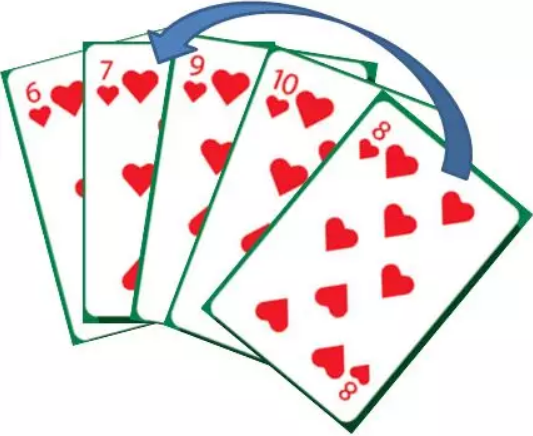
\includegraphics[scale=0.4]{img/C8/8-4/1.png}
	\caption{理牌}
\end{figure}

例如一个有8个数字组成的无序序列,进行升序排序。

\begin{figure}[H]
	\centering
	\begin{tikzpicture}[font=\ttfamily,
			array/.style={matrix of nodes,nodes={draw, minimum size=10mm, fill=green!30},column sep=-\pgflinewidth, row sep=0.5mm, nodes in empty cells,
					row 1/.style={nodes={draw=none, fill=none, minimum size=5mm}},
				}]

		\matrix[array] (array) {
			0 & 1 & 2 & 3 & 4 & 5 & 6 & 7 \\
			5 & 8 & 6 & 3 & 9 & 2 & 1 & 7 \\
			5 & 8 & 6 & 3 & 9 & 2 & 1 & 7 \\
			5 & 6 & 8 & 3 & 9 & 2 & 1 & 7 \\
			3 & 5 & 6 & 8 & 9 & 2 & 1 & 7 \\
			3 & 5 & 6 & 8 & 9 & 2 & 1 & 7 \\
			2 & 3 & 5 & 6 & 8 & 9 & 1 & 7 \\
			1 & 2 & 3 & 5 & 6 & 8 & 9 & 7 \\
			1 & 2 & 3 & 5 & 6 & 7 & 8 & 9 \\
		};

		\draw (-5,3.4) node{原数组};
		\draw (-5,2.4) node{第1轮};
		\draw (-5,1.3) node{第2轮};
		\draw (-5,0.2) node{第3轮};
		\draw (-5,-0.9) node{第4轮};
		\draw (-5,-1.9) node{第5轮};
		\draw (-5,-3) node{第6轮};
		\draw (-5,-4) node{第7轮};

		\draw[-, very thick, blue] (-4,3.9) rectangle (-3,2.95);
		\draw[-, very thick, blue] (-4,2.85) rectangle (-2,1.9);
		\draw[-, very thick, blue] (-4,1.8) rectangle (-1,0.8);
		\draw[-, very thick, blue] (-4,0.7) rectangle (0,-0.25);
		\draw[-, very thick, blue] (-4,-0.35) rectangle (1,-1.3);
		\draw[-, very thick, blue] (-4,-1.4) rectangle (2,-2.4);
		\draw[-, very thick, blue] (-4,-2.5) rectangle (3,-3.45);
		\draw[-, very thick, blue] (-4,-3.55) rectangle (4,-4.5);
	\end{tikzpicture}
	\caption{插入排序}
\end{figure}

\vspace{0.5cm}

\subsection{算法分析}

插入排序要进行n - 1轮,每一轮在最坏情况下的比较复制次数分别是1次、2次、3次、4次...一直到n - 1次,所以最坏时间复杂度是$ O(n^2) $。\\

至于空间复杂度,由于插入排序是在原地进行排序,并没有引入额外的数据结构,所以空间复杂度是$ O(1) $。

\begin{table}[H]
	\centering
	\setlength{\tabcolsep}{5mm}{
		\begin{tabular}{|c|c|c|c|}
			\hline
			\textbf{时间复杂度} & \textbf{空间复杂度} & \textbf{稳定性} & \textbf{设计思想} \\
			\hline
			$ O(n^2) $          & $ O(1) $            & 稳定            & 减治法            \\
			\hline
		\end{tabular}
	}
	\caption{插入排序算法分析}
\end{table}

\mybox{插入排序}

\begin{lstlisting}[language=C]
void insertionSort(int *arr, int n) {
    for(int i = 1; i < n; i++) {
        int temp = arr[i];
        int j = i - 1;
        while(j >= 0 && temp < arr[j]) {
            arr[j+1] = arr[j];
            j--;
        }
        arr[j+1] = temp;
    }
}
\end{lstlisting}

\vspace{0.5cm}

\subsection{折半插入排序(Binary Insertion Sort)}

折半插入排序是对插入排序的改进,其过程就是不断依次将元素插入前面已经排好序的序列中,在寻找插入点时采用了折半查找。\\

\mybox{折半插入排序}

\begin{lstlisting}[language=C]
void binaryInsertionSort(int *arr, int n) {
    for(int i = 1; i < n; i++) {
        int temp = arr[i];
        int start = 0;
        int end = i - 1;
        while(start <= end) {
            int mid = start + (end - start) / 2;
            if(arr[mid] > temp) {
                end = mid - 1;
            } else {
                start = mid + 1;
            }
        }
        int j;
        for(j = i - 1; j > end; j--) {
            arr[j+1] = arr[j];
        }
        arr[j+1] = temp;
    }
}
\end{lstlisting}

\newpage

\section{鸡尾酒排序}

\subsection{鸡尾酒排序(Cocktail Sort)}

对一个无序数组\{2, 3, 4, 5, 6, 7, 8, 1\}进行升序排序,如果按照冒泡排序,步骤如下:

\begin{figure}[H]
	\centering
	\begin{tikzpicture}[font=\ttfamily,
			array/.style={matrix of nodes,nodes={draw, minimum size=10mm, fill=green!30},column sep=-\pgflinewidth, row sep=0.5mm, nodes in empty cells,
					row 1/.style={nodes={draw=none, fill=none, minimum size=5mm}},
				}]

		\matrix[array] (array) {
			0 & 1 & 2 & 3 & 4 & 5 & 6 & 7 \\
			2 & 3 & 4 & 5 & 6 & 7 & 1 & 8 \\
			2 & 3 & 4 & 5 & 6 & 7 & 1 & 8 \\
			2 & 3 & 4 & 5 & 6 & 1 & 7 & 8 \\
			2 & 3 & 4 & 5 & 1 & 6 & 7 & 8 \\
			2 & 3 & 4 & 1 & 5 & 6 & 7 & 8 \\
			2 & 3 & 1 & 4 & 5 & 6 & 7 & 8 \\
			2 & 1 & 3 & 4 & 5 & 6 & 7 & 8 \\
			1 & 2 & 3 & 4 & 5 & 6 & 7 & 8 \\
		};

		\draw (-5,3.4) node{原数组};
		\draw (-5,2.4) node{第1轮};
		\draw (-5,1.3) node{第2轮};
		\draw (-5,0.2) node{第3轮};
		\draw (-5,-0.9) node{第4轮};
		\draw (-5,-1.9) node{第5轮};
		\draw (-5,-3) node{第6轮};
		\draw (-5,-4) node{第7轮};

		\draw[-, very thick, blue] (3,2.85) rectangle (4,1.9);
		\draw[-, very thick, blue] (2,1.8) rectangle (4,0.8);
		\draw[-, very thick, blue] (1,0.7) rectangle (4,-0.25);
		\draw[-, very thick, blue] (0,-0.35) rectangle (4,-1.3);
		\draw[-, very thick, blue] (-1,-1.4) rectangle (4,-2.4);
		\draw[-, very thick, blue] (-2,-2.5) rectangle (4,-3.45);
		\draw[-, very thick, blue] (-3,-3.55) rectangle (4,-4.5);
	\end{tikzpicture}
	\caption{冒泡排序}
\end{figure}

从2到8已经是有序了,只有元素1的位置不对,却还要进行7轮排序,这也太憋屈了吧!\\

鸡尾酒排序正是用于解决这种问题的。鸡尾酒排序又叫快乐小时排序,它基于冒泡排序做了一点小小的优化。\\

鸡尾酒排序的第一轮与冒泡排序相同,从左向右比较和交换。

\begin{figure}[H]
	\centering
	\begin{tikzpicture}[font=\ttfamily,
			array/.style={matrix of nodes,nodes={draw, minimum size=10mm, fill=green!30},column sep=-\pgflinewidth, row sep=0.5mm, nodes in empty cells,
					row 1/.style={nodes={draw=none, fill=none, minimum size=5mm}},
				}]

		\matrix[array] (array) {
			0 & 1 & 2 & 3 & 4 & 5 & 6 & 7 \\
			2 & 3 & 4 & 5 & 6 & 7 & 1 & 8 \\
		};

		\draw[-, very thick, blue] (3,0.2) rectangle (4,-0.8);
	\end{tikzpicture}
	\caption{鸡尾酒排序第1轮}
\end{figure}

第二轮开始不一样了,反过来向右向左比较和交换。

\begin{figure}[H]
	\centering
	\begin{tikzpicture}[font=\ttfamily,
			array/.style={matrix of nodes,nodes={draw, minimum size=10mm, fill=green!30},column sep=-\pgflinewidth, row sep=0.5mm, nodes in empty cells,
					row 1/.style={nodes={draw=none, fill=none, minimum size=5mm}},
				}]

		\matrix[array] (array) {
			0 & 1 & 2 & 3 & 4 & 5 & 6 & 7 \\
			2 & 3 & 4 & 5 & 6 & 7 & 1 & 8 \\
			2 & 3 & 4 & 5 & 6 & 1 & 7 & 8 \\
			2 & 3 & 4 & 5 & 1 & 6 & 7 & 8 \\
			2 & 3 & 4 & 1 & 5 & 6 & 7 & 8 \\
			2 & 3 & 1 & 4 & 5 & 6 & 7 & 8 \\
			2 & 1 & 3 & 4 & 5 & 6 & 7 & 8 \\
			1 & 2 & 3 & 4 & 5 & 6 & 7 & 8 \\
		};

		\draw[-, very thick, red] (1,3.4) rectangle (3,2.4);
		\draw[-, very thick, red] (0,2.3) rectangle (2,1.35);
		\draw[-, very thick, red] (-1,1.25) rectangle (1,0.28);
		\draw[-, very thick, red] (-2,0.2) rectangle (0,-0.8);
		\draw[-, very thick, red] (-3,-0.9) rectangle (-1,-1.85);
		\draw[-, very thick, red] (-4,-1.95) rectangle (-2,-2.9);

		\draw[<->, very thick, red] (1.65,2.87) -- (2.4,2.87);
		\draw[<->, very thick, red] (0.7,1.83) -- (1.4,1.83);
		\draw[<->, very thick, red] (-0.4,0.79) -- (0.4,0.79);
		\draw[<->, very thick, red] (-1.3,-0.3) -- (-0.6,-0.3);
		\draw[<->, very thick, red] (-2.3,-1.4) -- (-1.6,-1.4);
		\draw[<->, very thick, red] (-3.4,-2.45) -- (-2.6,-2.45);
	\end{tikzpicture}
	\caption{鸡尾酒排序第2轮}
\end{figure}

第二轮结束后,此时虽然已经有序,但是算法并没有结束。\\

第三轮再次从左向右比较和交换,在此过程中,没有元素发生交换,证明已经有序,排序结束。\\

鸡尾酒排序的过程就像钟摆一样,左右来回比较和交换。本来冒泡要用8轮排序的场景,鸡尾酒用3轮就解决了。\\

鸡尾酒排序的优点是能够在大部分元素已经有序的情况下,减少排序的回合数;而缺点也很明显,就是代码量几乎扩大了一倍。\\

\mybox{鸡尾酒排序}

\begin{lstlisting}[language=C]
void cocktailSort1(int *arr, int n) {
    for(int i = 0; i < n / 2; i++) {
        // 从左向右
        bool isSorted = true;   // 标记当前轮是否有序
        for(int j = i; j < n - i - 1; j++) {
            if(arr[j] > arr[j+1]) {
                swap(&arr[j], &arr[j+1]);
                isSorted = false;   // 发生交换
            }
        }
        if(isSorted) {
            break;
        }

        // 从右向左
        isSorted = true;
        for(int j = n - i - 1; j > i; j--) {
            if(arr[j] < arr[j-1]) {
                swap(&arr[j], &arr[j-1]);
                isSorted = false;
            }
        }
        if(isSorted) {
            break;
        }
    }
}
\end{lstlisting}

\vspace{0.5cm}

\subsection{鸡尾酒排序优化}

类似冒泡排序的优化方法,鸡尾酒排序也可以记录每一轮排序后最后一次元素交换的位置。但是对于双向的鸡尾酒排序而言,需要设置两个边界值。\\

\mybox{鸡尾酒排序优化}

\begin{lstlisting}[language=C]
void cocktailSort2(int *arr, int n) {
    int lastLeft = 0;           // 左侧最后一次交换位置
    int lastRight = 0;          // 右侧最后一次交换位置
    int leftBorder = 0;         // 无序区左边界
    int rightBorder = n - 1;    // 无序区右边界

    for(int i = 0; i < n / 2; i++) {
        // 从左向右
        bool isSorted = true;   // 标记当前轮是否有序
        for(int j = leftBorder; j < rightBorder; j++) {
            if(arr[j] > arr[j+1]) {
                swap(&arr[j], &arr[j+1]);
                isSorted = false;   // 发生交换
                lastRight = j;
            }
        }
        if(isSorted) {
            break;
        }
        rightBorder = lastRight;

        // 从右向左
        isSorted = true;
        for(int j = n - i - 1; j > i; j--) {
            if(arr[j] < arr[j-1]) {
                swap(&arr[j], &arr[j-1]);
                isSorted = false;
                lastLeft = j;
            }
        }
        if(isSorted) {
            break;
        }
        leftBorder = lastLeft;
    }
}
\end{lstlisting}

\newpage

\section{归并排序}

\subsection{归并排序(Merge Sort)}

归并排序算法采用分治法:

\begin{enumerate}
	\item 分解:将序列每次折半划分。
	\item 合并:将划分后的序列两两按序合并。
\end{enumerate}

\begin{figure}[H]
	\centering
	\begin{tikzpicture}[level distance=1.2cm,
			level 1/.style={sibling distance=4cm},
			level 2/.style={sibling distance=2cm},
			level 3/.style={sibling distance=1cm},
			edgedown/.style={edge from parent/.style={draw=red,thick,-latex}},
			edgeup/.style={edge from parent/.style={draw=green!50!black,thick,latex-}}
		]

		\node[gblock=7,yshift=-7.2cm] (A') {3 \nodepart{two} 9 \nodepart{three} 10 \nodepart{four} 27 \nodepart{five} 39 \nodepart{six}43 \nodepart{seven}82}
		[grow=up,edgeup]
		child {node[gblock=3] (B2') {9 \nodepart{two} 10 \nodepart{three} 82}
				child {node[gblock=1] (C4') {10}
						child {node[gblock=1] (D7') {10}}
					}
				child {node[gblock=2] (C2') {9 \nodepart{two} 82}
						child {node[gblock=1] (D3') {82}}
						child {node[gblock=1] (D4') {9}}
					}
			}
		child {node[gblock=4] (B1') {3 \nodepart{two} 27 \nodepart{three} 39 \nodepart{four} 43}
				child {node[gblock=2] (C3') {3 \nodepart{two} 43}
						child {node[gblock=1] (D5') {3}}
						child {node[gblock=1] (D6') {43}}
					}
				child {node[gblock=2] (C1') {27 \nodepart{two} 39}
						child {node[gblock=1] (D1') {27}}
						child {node[gblock=1] (D2') {39}}
					}
			};

		\node[block=7] (A) {39 \nodepart{two} 27 \nodepart{three} 43 \nodepart{four} 3 \nodepart{five} 9 \nodepart{six}82 \nodepart{seven}10}
		[grow=down,edgedown]
		child {node[block=4] (B1) {39 \nodepart{two} 27 \nodepart{three} 43 \nodepart{four} 3}
				child {node[block=2] (C1) {39 \nodepart{two} 27}
						child {node[block=1] (D1) {39}}
						child {node[block=1] (D2) {27}}
					}
				child {node[block=2] (C2) {43 \nodepart{two} 3}
						child {node[block=1] (D3) {43}}
						child {node[block=1] (D4) {3}}
					}
			}
		child {node[block=3] (B2) {9 \nodepart{two} 82 \nodepart{three} 10}
				child {node[block=2] (C3) {9 \nodepart{two} 82}
						child {node[block=1] (D5) {9}}
						child {node[block=1] (D6) {82}}
					}
				child {node[block=1] (C4) {10}
						child {node[block=1] (D7) {10}}
					}
			};
	\end{tikzpicture}
	\caption{归并排序}
\end{figure}

\vspace{0.5cm}

\subsection{算法分析}

归并排序每次将数组折半对分,一共分了$ logn $次,每一层进行合并操作的运算量是n,所以时间复杂度为$ O(nlogn) $。归并排序的速度仅次于快速排序。\\

\begin{table}[H]
	\centering
	\setlength{\tabcolsep}{5mm}{
		\begin{tabular}{|c|c|c|c|}
			\hline
			\textbf{时间复杂度} & \textbf{空间复杂度} & \textbf{稳定性} & \textbf{设计思想} \\
			\hline
			$ O(nlogn) $        & $ O(n) $            & 稳定            & 分治法            \\
			\hline
		\end{tabular}
	}
	\caption{归并排序算法分析}
\end{table}

\mybox{归并排序}

\begin{lstlisting}[language=C]
void merge(int *arr, int start, int mid, int end, int *temp) {
    int i = start;
    int j = mid + 1;
    int k = 0;

    while(i <= mid && j <= end) {
        if(arr[i] <= arr[j]) {
            temp[k++] = arr[i++];
        } else {
            temp[k++] = arr[j++];
        }
    }

    while(i <= mid) {
        temp[k++] = arr[i++];
    }
    while(j <= end) {
        temp[k++] = arr[j++];
    }

    for(int i = 0; i < k; i++) {
        arr[start+i] = temp[i];
    }
}

void mergeSort(int *arr, int start, int end, int *temp) {
    if(start < end) {
        int mid = start + (end - start) / 2;
        mergeSort(arr, start, mid, temp);
        mergeSort(arr, mid+1, end, temp);
        merge(arr, start, mid, end, temp);
    }
}
\end{lstlisting}

\newpage

\section{快速排序}

\subsection{快速排序(Quick Sort)}

快速排序是很重要的算法,与傅里叶变换等算法并称二十世纪十大算法。\\

快速排序之所以快,是因为它使用了分治法。快速排序在每一轮挑选一个基准(pivot)元素,并让其它比它小的元素移动到数列一边,比它大的元素移动到数列的另一边,从而把数列拆解成了两个部分。\\

选择基准元素最简单的方式是选择数列的第一个元素。这种选择在绝大多数情况下是没有问题的,但是如果对一个原本逆序的数列进行升序排序,整个数列并没有被分成一半,每一轮仅仅确定了基准元素的位置。这种情况下数列第一个元素要么是最小值,要么是最大值,根本无法发挥分治法的优势。在这种极端情况下,快速排序需要进行n轮,时间复杂度退化成了$ O(n^2) $。

如何避免这种极端情况呢?可以不选择数列的第一个元素,而是随机选择一个元素作为基准元素。这样一来,即使是在数列完全逆序的情况下,也可以有效地将数列分成两部分。当然,即使是随机选择,每一次也有极小的几率选到数列的最大值或最小值,同样会对分治造成一定影响。\\

确定了基准值后,如何实现将小于基准的元素都移动到基准值一边,大于基准值的都移动到另一边呢?\\

例如一个有8个数字组成的无序序列,进行升序排序。选定基准元素pivot,设置两个指针left和right,指向数列的最左和最右两个元素。

\begin{figure}[H]
	\centering
	\begin{tikzpicture}[font=\ttfamily,
			array/.style={matrix of nodes,nodes={draw, minimum size=10mm, fill=green!30},column sep=-\pgflinewidth, row sep=0.5mm, nodes in empty cells,
					row 1/.style={nodes={draw=none, fill=none, minimum size=5mm}},
				}]

		\matrix[array] (array) {
			0 & 1 & 2 & 3 & 4 & 5 & 6 & 7 \\
			4 & 7 & 6 & 5 & 3 & 2 & 8 & 1 \\
		};

		\draw (-5.5,-0.3) node{pivot = 4};
		\draw[-, very thick, red] (-4,0.2) rectangle (-3,-0.8);
		\draw (-3.5,-1.3) node{left};
		\draw (3.5,-1.3) node{right};
	\end{tikzpicture}
\end{figure}

从right指针开始,把指针所指向的元素和基准元素做比较。如果比pivot大,则right指针向左移动;如果比pivot小,则把right所指向的元素填入left指针所指向的位置,同时left向右移动一位。

\begin{figure}[H]
	\centering
	\begin{tikzpicture}[font=\ttfamily,
			array/.style={matrix of nodes,nodes={draw, minimum size=10mm, fill=green!30},column sep=-\pgflinewidth, row sep=0.5mm, nodes in empty cells,
					row 1/.style={nodes={draw=none, fill=none, minimum size=5mm}},
				}]

		\matrix[array] (array) {
			0 & 1 & 2 & 3 & 4 & 5 & 6 & 7 \\
			1 & 7 & 6 & 5 & 3 & 2 & 8 & 1 \\
		};

		\draw (-5.5,-0.3) node{pivot = 4};
		\draw[-, very thick, blue] (-4,0.2) rectangle (-3,-0.8);
		\draw (-2.5,-1.3) node{left};
		\draw (3.5,-1.3) node{right};
	\end{tikzpicture}
\end{figure}

接着,切换到left指针进行比较,把指针所指向的元素和基准元素做比较。如果小于pivot,则left指针向右移动;如果大于pivot,则把left所指向的元素填入right指针所指向的位置,同时right向左移动一位。

\begin{figure}[H]
	\centering
	\begin{tikzpicture}[font=\ttfamily,
			array/.style={matrix of nodes,nodes={draw, minimum size=10mm, fill=green!30},column sep=-\pgflinewidth, row sep=0.5mm, nodes in empty cells,
					row 1/.style={nodes={draw=none, fill=none, minimum size=5mm}},
				}]

		\matrix[array] (array) {
			0 & 1 & 2 & 3 & 4 & 5 & 6 & 7 \\
			1 & 7 & 6 & 5 & 3 & 2 & 8 & 7 \\
		};

		\draw (-5.5,-0.3) node{pivot = 4};
		\draw[-, very thick, blue] (-4,0.2) rectangle (-3,-0.8);
		\draw[-, very thick, orange] (3,0.2) rectangle (4,-0.8);
		\draw (-2.5,-1.3) node{left};
		\draw (2.5,-1.3) node{right};
	\end{tikzpicture}
\end{figure}

重复之前的步骤继续排序:

\begin{figure}[H]
	\centering
	\begin{tikzpicture}[font=\ttfamily,
			array/.style={matrix of nodes,nodes={draw, minimum size=10mm, fill=green!30},column sep=-\pgflinewidth, row sep=0.5mm, nodes in empty cells,
					row 1/.style={nodes={draw=none, fill=none, minimum size=5mm}},
				}]

		\matrix[array] (array) {
			0 & 1 & 2 & 3 & 4 & 5 & 6 & 7 \\
			1 & 7 & 6 & 5 & 3 & 2 & 8 & 7 \\
		};

		\draw (-5.5,-0.3) node{pivot = 4};
		\draw[-, very thick, blue] (-4,0.2) rectangle (-3,-0.8);
		\draw[-, very thick, orange] (2,0.2) rectangle (4,-0.8);
		\draw (-2.5,-1.3) node{left};
		\draw (1.5,-1.3) node{right};
	\end{tikzpicture}

	\begin{tikzpicture}[font=\ttfamily,
			array/.style={matrix of nodes,nodes={draw, minimum size=10mm, fill=green!30},column sep=-\pgflinewidth, row sep=0.5mm, nodes in empty cells,
					row 1/.style={nodes={draw=none, fill=none, minimum size=5mm}},
				}]

		\matrix[array] (array) {
			0 & 1 & 2 & 3 & 4 & 5 & 6 & 7 \\
			1 & 2 & 6 & 5 & 3 & 2 & 8 & 7 \\
		};

		\draw (-5.5,-0.3) node{pivot = 4};
		\draw[-, very thick, blue] (-4,0.2) rectangle (-2,-0.8);
		\draw[-, very thick, orange] (2,0.2) rectangle (4,-0.8);
		\draw (-1.5,-1.3) node{left};
		\draw (1.5,-1.3) node{right};
	\end{tikzpicture}

	\begin{tikzpicture}[font=\ttfamily,
			array/.style={matrix of nodes,nodes={draw, minimum size=10mm, fill=green!30},column sep=-\pgflinewidth, row sep=0.5mm, nodes in empty cells,
					row 1/.style={nodes={draw=none, fill=none, minimum size=5mm}},
				}]

		\matrix[array] (array) {
			0 & 1 & 2 & 3 & 4 & 5 & 6 & 7 \\
			1 & 2 & 6 & 5 & 3 & 6 & 8 & 7 \\
		};

		\draw (-5.5,-0.3) node{pivot = 4};
		\draw[-, very thick, blue] (-4,0.2) rectangle (-2,-0.8);
		\draw[-, very thick, orange] (1,0.2) rectangle (4,-0.8);
		\draw (-1.5,-1.3) node{left};
		\draw (0.5,-1.3) node{right};
	\end{tikzpicture}

	\begin{tikzpicture}[font=\ttfamily,
			array/.style={matrix of nodes,nodes={draw, minimum size=10mm, fill=green!30},column sep=-\pgflinewidth, row sep=0.5mm, nodes in empty cells,
					row 1/.style={nodes={draw=none, fill=none, minimum size=5mm}},
				}]

		\matrix[array] (array) {
			0 & 1 & 2 & 3 & 4 & 5 & 6 & 7 \\
			1 & 2 & 3 & 5 & 3 & 6 & 8 & 7 \\
		};

		\draw (-5.5,-0.3) node{pivot = 4};
		\draw[-, very thick, blue] (-4,0.2) rectangle (-1,-0.8);
		\draw[-, very thick, orange] (1,0.2) rectangle (4,-0.8);
		\draw (-0.5,-1.3) node{left};
		\draw (0.5,-1.3) node{right};
	\end{tikzpicture}

	\begin{tikzpicture}[font=\ttfamily,
			array/.style={matrix of nodes,nodes={draw, minimum size=10mm, fill=green!30},column sep=-\pgflinewidth, row sep=0.5mm, nodes in empty cells,
					row 1/.style={nodes={draw=none, fill=none, minimum size=5mm}},
				}]

		\matrix[array] (array) {
			0 & 1 & 2 & 3 & 4 & 5 & 6 & 7 \\
			1 & 2 & 3 & 5 & 5 & 6 & 8 & 7 \\
		};

		\draw (-5.5,-0.3) node{pivot = 4};
		\draw[-, very thick, blue] (-4,0.2) rectangle (-1,-0.8);
		\draw[-, very thick, orange] (0,0.2) rectangle (4,-0.8);
		\draw[-, very thick, red] (-1,0.2) rectangle (0,-0.8);
		\draw (-0.5,-1.3) node{left};
		\draw (-0.5,-2) node{right};
	\end{tikzpicture}
\end{figure}

当left和right指针重合在同一位置的时候,把之前的pivot元素的值填入该重合的位置。此时数列左边的元素都小于基准元素,数列右边的元素都大于基准元素。\\

\subsection{算法分析}

分治法的思想下,原数列在每一轮被拆分成两部分,每一部分在下一轮又被拆分成两部分,直到不可再分为止。这样平均情况下需要$ logn $轮,因此快速排序算法的平均时间复杂度是$ O(nlogn) $。

\begin{table}[H]
	\centering
	\setlength{\tabcolsep}{5mm}{
		\begin{tabular}{|c|c|c|c|}
			\hline
			\textbf{时间复杂度}      & \textbf{空间复杂度}   & \textbf{稳定性} & \textbf{设计思想} \\
			\hline
			$ O(nlogn) \sim O(n^2) $ & $ O(logn) \sim O(n) $ & 不稳定          & 分治法            \\
			\hline
		\end{tabular}
	}
	\caption{快速排序算法分析}
\end{table}

\mybox{快速排序}

\begin{lstlisting}[language=C]
void quickSort(int *arr, int start, int end) {
    if(start < end) {
        int i = start;
        int j = end;
        int pivot = arr[start];

        while(i < j) {
            while(i < j && arr[j] > pivot) {
                j--;
            }
            if(i < j) {
                arr[i] = arr[j];
                i++;
            }
            while(i < j && arr[i] < pivot) {
                i++;
            }
            if(i < j) {
                arr[j] = arr[i];
                j--;
            }
        }
        arr[i] = pivot;
        quickSort(arr, start, i-1);
        quickSort(arr, i+1, end);
    } 
}
\end{lstlisting}

\newpage

\section{计数排序}

\subsection{计数排序(Counting Sort)}

基于比较的排序算法的最优下界为$ \Omega(nlogn) $。计数排序是一种不基于比较的排序算法,而是利用数组下标来确定元素的正确位置。\\

遍历数列,将每一个整数按照其值对号入座,对应数组下标的元素加1。数组的每一个下标位置的值,代表了数列中对应整数出现的次数。有了这个统计结果,直接遍历数组,输出数组元素的下标值,元素的值是多少就输出多少次。\\

从功能角度,这个算法可以实现整数的排序,但是也存在一些问题。如果只以最大值来决定统计数组的长度并不严谨,例如数列\{95, 94, 91, 98, 99, 90, 99, 93, 91, 92\},这个数列的最大值是99,但最小值是90。如果创建长度为100的数组,前面的从0到89的空间位置都浪费了。\\

因此,不应再以数列的max + 1作为统计数组的长度,而是以数列max - min + 1作为统计数组的长度。同时,数列的最小值作为一个偏移量,用于统计数组的对号入座。\\

计数排序适用于一定范围的整数排序,在取值范围不是很大的情况下,它的性能甚至快过那些$ O(nlogn) $的排序算法。\\

\mybox{计数排序}

\begin{lstlisting}[language=C]
void countingSort(int *arr, int n) {
    int max = arr[0];
    int min = arr[0];
    for(int i = 1; i < n; i++) {
        if(arr[i] > max) {
            max = arr[i];
        }
        if(arr[i] < min) {
            min = arr[i];
        }
    }
    
    int range = max - min + 1;
    int table[range];
    memset(table, 0, sizeof(table));

    for(int i = 0; i < n; i++) {
        table[arr[i] - min]++;
    }

    int cnt = 0;
    for(int i = 0; i < range; i++) {
        while(table[i]--) {
            arr[cnt++] = i + min;
        }
    }
}
\end{lstlisting}

\newpage

\section{桶排序}

\subsection{桶排序(Bucket Sort)}

桶排序是计数排序的扩展版本。计数排序可以看成每个桶只存储相同元素,而桶排序每个桶存储一定范围的元素。\\

每一个桶代表一个区间范围,里面可以承载一个或多个元素。通过划分多个范围相同的区间,将每个子区间自排序,最后合并。桶排序需要尽量保证元素分散均匀,否则当所有数据集中在同一个桶中时,桶排序失效。\\

例如一个待排序的序列:

\begin{figure}[H]
	\centering
	\begin{tikzpicture}[font=\ttfamily,
			array/.style={matrix of nodes,nodes={draw, minimum size=10mm, fill=green!30},column sep=-\pgflinewidth, row sep=0.5mm, nodes in empty cells,
					row 1/.style={nodes={draw=none, fill=none, minimum size=5mm}},
				}]

		\matrix[array] (array) {
			0  & 1  & 2  & 3  & 4  & 5  \\
			18 & 11 & 28 & 45 & 23 & 50 \\
		};
	\end{tikzpicture}
\end{figure}

确定桶的个数与每个桶的取值范围,遍历待排序序列,将元素放入对应的桶中:

\begin{figure}[H]
	\centering
	\begin{tikzpicture}
		\node (a) [cylinder, xshift=0cm, shape border rotate=90, draw, minimum height=20mm, minimum width=15mm] {};
		\node (b) [cylinder, xshift=2cm, shape border rotate=90, draw, minimum height=20mm, minimum width=15mm] {};
		\node (c) [cylinder, xshift=4cm, shape border rotate=90, draw, minimum height=20mm, minimum width=15mm] {};
		\node (d) [cylinder, xshift=6cm, shape border rotate=90, draw, minimum height=20mm, minimum width=15mm] {};

		\draw (0,-1.5) node{$ [10, 20) $};
			\draw (2,-1.5) node{$ [20, 30) $};
		\draw (4,-1.5) node{$ [30, 40) $};
			\draw (6,-1.5) node{$ [40, 50) $};

		\draw (0,0) node{18};
		\draw (0,-0.5) node{11};
		\draw (2,0) node{28};
		\draw (2,-0.5) node{23};
		\draw (6,0) node{45};
		\draw (6,-0.5) node{50};
	\end{tikzpicture}
\end{figure}

分别对每个桶中的元素进行排序:

\begin{figure}[H]
	\centering
	\begin{tikzpicture}
		\node (a) [cylinder, xshift=0cm, shape border rotate=90, draw, minimum height=20mm, minimum width=15mm] {};
		\node (b) [cylinder, xshift=2cm, shape border rotate=90, draw, minimum height=20mm, minimum width=15mm] {};
		\node (c) [cylinder, xshift=4cm, shape border rotate=90, draw, minimum height=20mm, minimum width=15mm] {};
		\node (d) [cylinder, xshift=6cm, shape border rotate=90, draw, minimum height=20mm, minimum width=15mm] {};

		\draw (0,-1.5) node{$ [10, 20) $};
			\draw (2,-1.5) node{$ [20, 30) $};
		\draw (4,-1.5) node{$ [30, 40) $};
			\draw (6,-1.5) node{$ [40, 50) $};

		\draw (0,0) node{11};
		\draw (0,-0.5) node{18};
		\draw (2,0) node{23};
		\draw (2,-0.5) node{28};
		\draw (6,0) node{45};
		\draw (6,-0.5) node{50};
	\end{tikzpicture}
\end{figure}

将桶中的元素按顺序赋值到原始数组中:

\begin{figure}[H]
	\centering
	\begin{tikzpicture}[font=\ttfamily,
			array/.style={matrix of nodes,nodes={draw, minimum size=10mm, fill=green!30},column sep=-\pgflinewidth, row sep=0.5mm, nodes in empty cells,
					row 1/.style={nodes={draw=none, fill=none, minimum size=5mm}},
				}]

		\matrix[array] (array) {
			0  & 1  & 2  & 3  & 4  & 5  \\
			11 & 18 & 23 & 28 & 45 & 50 \\
		};
	\end{tikzpicture}
\end{figure}

创建桶的数量取决于数据的区间范围,一般创建桶的数量等于待排序的元素数量,每个桶的区间跨度为:

$$
	max - min \over buckets - 1
$$

\vspace{0.5cm}

\mybox{桶排序}

\begin{lstlisting}[language=Java]
public static void bucketSort(int[] arr) {
        int max = arr[0];
        int min = arr[0];
        for(int i = 1; i < arr.length; i++) {
            if(arr[i] > max) {
                max = arr[i];
            }
            if(arr[i] < min) {
                min = arr[i];
            }
        }
        int diff = max - min;

        // 创建桶
        int bucketNum = arr.length;
        List<LinkedList<Integer>> buckets 
            = new ArrayList<>(bucketNum);
        for(int i = 0; i < bucketNum; i++) {
            buckets.add(new LinkedList<>());
        }

        // 遍历数组,把元素放入对应桶中
        for(int i = 0; i < arr.length; i++) {
            // 计算当前元素所放置的桶号
            int num = (arr[i]-min) / (diff / (bucketNum-1));
            buckets.get(num).add(arr[i]);
        }

        // 桶内排序
        for(int i = 0; i < bucketNum; i++) {
            Collections.sort(buckets.get(i));
        }

        // 取出元素
        int cnt = 0;
        for(LinkedList<Integer> list : buckets) {
            for(int data : list) {
                arr[cnt++] = data;
            }
        }
    }
\end{lstlisting}

\newpage

\section{基数排序}

\subsection{基数排序(Radix Sort)}

基数排序可以看作是桶排序的扩展,主要思想是将整数按位划分。\\

基数排序需要准备10个桶,分别代表0 $ \sim $ 9,根据整数个位数字的数值将元素放入对应的桶中,之后按照输入赋值到原序列中,再依次对十位、百位等进行同样的操作。

例如一个待排序的序列:

\begin{figure}[H]
	\centering
	\begin{tikzpicture}[font=\ttfamily,
			array/.style={matrix of nodes,nodes={draw, minimum size=10mm, fill=green!30},column sep=-\pgflinewidth, row sep=0.5mm, nodes in empty cells,
					row 1/.style={nodes={draw=none, fill=none, minimum size=5mm}},
				}]

		\matrix[array] (array) {
			0 & 1 & 2  & 3  & 4  & 5  & 6  & 7  & 8  \\
			3 & 1 & 18 & 11 & 28 & 45 & 23 & 50 & 30 \\
		};
	\end{tikzpicture}
\end{figure}

根据个位数值放入对应的桶中:

\begin{figure}[H]
	\centering
	\begin{tikzpicture}
		\node (a) [cylinder, xshift=0cm, shape border rotate=90, draw, minimum height=15mm, minimum width=10mm] {};
		\node (b) [cylinder, xshift=1.5cm, shape border rotate=90, draw, minimum height=15mm, minimum width=10mm] {};
		\node (c) [cylinder, xshift=3cm, shape border rotate=90, draw, minimum height=15mm, minimum width=10mm] {};
		\node (d) [cylinder, xshift=4.5cm, shape border rotate=90, draw, minimum height=15mm, minimum width=10mm] {};
		\node (e) [cylinder, xshift=6cm, shape border rotate=90, draw, minimum height=15mm, minimum width=10mm] {};
		\node (f) [cylinder, xshift=7.5cm, shape border rotate=90, draw, minimum height=15mm, minimum width=10mm] {};
		\node (g) [cylinder, xshift=9cm, shape border rotate=90, draw, minimum height=15mm, minimum width=10mm] {};
		\node (h) [cylinder, xshift=10.5cm, shape border rotate=90, draw, minimum height=15mm, minimum width=10mm] {};
		\node (i) [cylinder, xshift=12cm, shape border rotate=90, draw, minimum height=15mm, minimum width=10mm] {};
		\node (j) [cylinder, xshift=13.5cm, shape border rotate=90, draw, minimum height=15mm, minimum width=10mm] {};

		\draw (0,-1) node{0};
		\draw (1.5,-1) node{1};
		\draw (3,-1) node{2};
		\draw (4.5,-1) node{3};
		\draw (6,-1) node{4};
		\draw (7.5,-1) node{5};
		\draw (9,-1) node{6};
		\draw (10.5,-1) node{7};
		\draw (12,-1) node{8};
		\draw (13.5,-1) node{9};

		\draw (0,0.3) node{50};
		\draw (0,-0.3) node{30};
		\draw (1.5,0.3) node{1};
		\draw (1.5,-0.3) node{11};
		\draw (4.5,0.3) node{3};
		\draw (4.5,-0.3) node{23};
		\draw (7.5,-0.3) node{45};
		\draw (12,0.3) node{18};
		\draw (12,-0.3) node{28};
	\end{tikzpicture}
\end{figure}

将桶中的元素按顺序赋值到原始数组中:

\begin{figure}[H]
	\centering
	\begin{tikzpicture}[font=\ttfamily,
			array/.style={matrix of nodes,nodes={draw, minimum size=10mm, fill=green!30},column sep=-\pgflinewidth, row sep=0.5mm, nodes in empty cells,
					row 1/.style={nodes={draw=none, fill=none, minimum size=5mm}},
				}]

		\matrix[array] (array) {
			0  & 1  & 2 & 3  & 4 & 5  & 6  & 7  & 8  \\
			50 & 30 & 1 & 11 & 3 & 23 & 45 & 18 & 28 \\
		};
	\end{tikzpicture}
\end{figure}

根据十位数值放入对应的桶中:

\begin{figure}[H]
	\centering
	\begin{tikzpicture}
		\node (a) [cylinder, xshift=0cm, shape border rotate=90, draw, minimum height=15mm, minimum width=10mm] {};
		\node (b) [cylinder, xshift=1.5cm, shape border rotate=90, draw, minimum height=15mm, minimum width=10mm] {};
		\node (c) [cylinder, xshift=3cm, shape border rotate=90, draw, minimum height=15mm, minimum width=10mm] {};
		\node (d) [cylinder, xshift=4.5cm, shape border rotate=90, draw, minimum height=15mm, minimum width=10mm] {};
		\node (e) [cylinder, xshift=6cm, shape border rotate=90, draw, minimum height=15mm, minimum width=10mm] {};
		\node (f) [cylinder, xshift=7.5cm, shape border rotate=90, draw, minimum height=15mm, minimum width=10mm] {};
		\node (g) [cylinder, xshift=9cm, shape border rotate=90, draw, minimum height=15mm, minimum width=10mm] {};
		\node (h) [cylinder, xshift=10.5cm, shape border rotate=90, draw, minimum height=15mm, minimum width=10mm] {};
		\node (i) [cylinder, xshift=12cm, shape border rotate=90, draw, minimum height=15mm, minimum width=10mm] {};
		\node (j) [cylinder, xshift=13.5cm, shape border rotate=90, draw, minimum height=15mm, minimum width=10mm] {};

		\draw (0,-1) node{0};
		\draw (1.5,-1) node{1};
		\draw (3,-1) node{2};
		\draw (4.5,-1) node{3};
		\draw (6,-1) node{4};
		\draw (7.5,-1) node{5};
		\draw (9,-1) node{6};
		\draw (10.5,-1) node{7};
		\draw (12,-1) node{8};
		\draw (13.5,-1) node{9};

		\draw (0,0.3) node{1};
		\draw (0,-0.3) node{3};
		\draw (1.5,0.3) node{11};
		\draw (1.5,-0.3) node{18};
		\draw (3,0.3) node{23};
		\draw (3,-0.3) node{28};
		\draw (4.5,0.3) node{30};
		\draw (4.5,-0.3) node{45};
		\draw (6,-0.3) node{50};
	\end{tikzpicture}
\end{figure}

将桶中的元素按顺序赋值到原始数组中:

\begin{figure}[H]
	\centering
	\begin{tikzpicture}[font=\ttfamily,
			array/.style={matrix of nodes,nodes={draw, minimum size=10mm, fill=green!30},column sep=-\pgflinewidth, row sep=0.5mm, nodes in empty cells,
					row 1/.style={nodes={draw=none, fill=none, minimum size=5mm}},
				}]

		\matrix[array] (array) {
			0 & 1 & 2  & 3  & 4  & 5  & 6  & 7  & 8  \\
			1 & 3 & 11 & 18 & 23 & 28 & 30 & 45 & 50 \\
		};
	\end{tikzpicture}
\end{figure}

\mybox{基数排序}

\begin{lstlisting}[language=Java]
public static void radixSort(int[] arr) {
        int max = arr[0];
        for(int i = 1; i < arr.length; i++) {
            if(arr[i] > max) {
                max = arr[i];
            }
        }

        int bucketNum = 10;
        // 从个位开始
        for(int exp = 1; max / exp > 0; exp *= 10) {
            // 创建桶
            List<LinkedList<Integer>> buckets 
                = new ArrayList<>(bucketNum);
            for(int i = 0; i < bucketNum; i++) {
                buckets.add(new LinkedList<>());
            }

            // 把元素放到对应桶中
            for(int data : arr) {
                int num = (data / exp) % 10;
                buckets.get(num).add(data);
            }

            // 按顺序取出元素
            int cnt = 0;
            for(LinkedList<Integer> bucket : buckets) {
                for(int data : bucket) {
                    arr[cnt++] = data;
                }
            }
        }
    }
\end{lstlisting}

\newpage

\section{珠排序}

\subsection{珠排序(Bead Sort)}

珠排序的算法和算盘非常类似。算盘上有许多圆圆的珠子被串在细杆上,如果把算盘竖起来,算盘上的小珠子会在重力的作用下滑到算盘底部。其中有一个很神奇的细节,如果统计每一横排珠子的数量,下落之后每一排珠子数量正好是下落前珠子数量的升序排序。

\begin{figure}[H]
	\centering
	\begin{tikzpicture}
		\draw[-, very thick] (0,0) -- (0,5);
		\draw[-, very thick] (1,0) -- (1,5);
		\draw[-, very thick] (2,0) -- (2,5);
		\draw[-, very thick] (3,0) -- (3,5);
		\draw[-, very thick] (4,0) -- (4,5);

		\draw (-1,4.5) node{3个};
		\draw (-1,3.5) node{2个};
		\draw (-1,2.5) node{4个};
		\draw (-1,1.5) node{5个};
		\draw (-1,0.5) node{1个};

		\draw[fill=brown] (0,4.5) circle (0.3);
		\draw[fill=brown] (0,3.5) circle (0.3);
		\draw[fill=brown] (0,2.5) circle (0.3);
		\draw[fill=brown] (0,1.5) circle (0.3);
		\draw[fill=brown] (0,0.5) circle (0.3);

		\draw[fill=brown] (1,4.5) circle (0.3);
		\draw[fill=brown] (1,3.5) circle (0.3);
		\draw[fill=brown] (1,2.5) circle (0.3);
		\draw[fill=brown] (1,1.5) circle (0.3);

		\draw[fill=brown] (2,4.5) circle (0.3);
		\draw[fill=brown] (2,2.5) circle (0.3);
		\draw[fill=brown] (2,1.5) circle (0.3);

		\draw[fill=brown] (3,2.5) circle (0.3);
		\draw[fill=brown] (3,1.5) circle (0.3);

		\draw[fill=brown] (4,1.5) circle (0.3);
	\end{tikzpicture}
\end{figure}

\begin{figure}[H]
	\centering
	\begin{tikzpicture}
		\draw[-, very thick] (0,0) -- (0,5);
		\draw[-, very thick] (1,0) -- (1,5);
		\draw[-, very thick] (2,0) -- (2,5);
		\draw[-, very thick] (3,0) -- (3,5);
		\draw[-, very thick] (4,0) -- (4,5);

		\draw (-1,4.5) node{1个};
		\draw (-1,3.5) node{2个};
		\draw (-1,2.5) node{3个};
		\draw (-1,1.5) node{4个};
		\draw (-1,0.5) node{5个};

		\draw[fill=brown] (0,4.5) circle (0.3);
		\draw[fill=brown] (0,3.5) circle (0.3);
		\draw[fill=brown] (0,2.5) circle (0.3);
		\draw[fill=brown] (0,1.5) circle (0.3);
		\draw[fill=brown] (0,0.5) circle (0.3);

		\draw[fill=brown] (1,3.5) circle (0.3);
		\draw[fill=brown] (1,2.5) circle (0.3);
		\draw[fill=brown] (1,1.5) circle (0.3);
		\draw[fill=brown] (1,0.5) circle (0.3);

		\draw[fill=brown] (2,2.5) circle (0.3);
		\draw[fill=brown] (2,1.5) circle (0.3);
		\draw[fill=brown] (2,0.5) circle (0.3);

		\draw[fill=brown] (3,1.5) circle (0.3);
		\draw[fill=brown] (3,0.5) circle (0.3);

		\draw[fill=brown] (4,0.5) circle (0.3);
	\end{tikzpicture}
	\caption{珠子下落}
\end{figure}

通过模拟珠子下落的元素可以对一组正整数进行排序。使用二维数组来模拟算盘,有珠子的位置设为1,没有珠子的位置设为0。例如一个有5个数字组成的无序整型数组\{3, 2, 4, 5, 1\}就可以转化为以下的二维数组:

\begin{table}[H]
	\centering
	\setlength{\tabcolsep}{5mm}{
		\begin{tabular}{|c|c|c|c|c|}
			\hline
			1 & 1 & 1 & 0 & 0 \\
			\hline
			1 & 1 & 0 & 0 & 0 \\
			\hline
			1 & 1 & 1 & 1 & 0 \\
			\hline
			1 & 1 & 1 & 1 & 1 \\
			\hline
			1 & 0 & 0 & 0 & 0 \\
			\hline
		\end{tabular}
	}
	\caption{模拟算盘}
\end{table}

接下来模拟算盘珠子掉落的过程,让所有的元素1都落到二维数组的最底部。

\begin{table}[H]
	\centering
	\setlength{\tabcolsep}{5mm}{
		\begin{tabular}{|c|c|c|c|c|}
			\hline
			1 & 0 & 0 & 0 & 0 \\
			\hline
			1 & 1 & 0 & 0 & 0 \\
			\hline
			1 & 1 & 1 & 0 & 0 \\
			\hline
			1 & 1 & 1 & 1 & 0 \\
			\hline
			1 & 1 & 1 & 1 & 1 \\
			\hline
		\end{tabular}
	}
\end{table}

最后把掉落后的算盘转换为一维有序数组\{1, 2, 3, 4, 5\}。

\newpage

\section{猴子排序}

\subsection{猴子排序(Bogo Sort)}

听说过“猴子和打字机”的理论吗?\\

无限猴子定理(Infinite Monkey Theorem)与薛定谔的猫、电车实验等并居十大思想实验,所谓思想实验即用想象力去进行,而在现实中基本无法去实现的实验。\\

无限猴子定理讲的是如果让一只猴子在打字机上胡乱打字,只要有无限的时间,总有一天可以恰好打出莎士比亚的著作。如果让无限只猴子在无限的空间、无限的时间里不停地敲打打字机,总有一天可以完整打出一本《哈姆雷特》,甚至是可以打出所有可能的文章。

\begin{figure}[H]
	\centering
	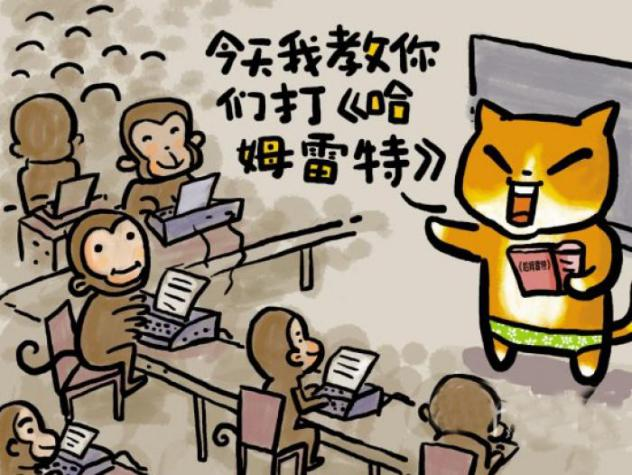
\includegraphics[]{img/C8/8-12/1.png}
	\caption{无限猴子定理}
\end{figure}

这个看似不可能的事情,却可以用现有数学原理被推导出来。但在现实中往往被认为是无法实现的,因为人们认为“无限”这个条件通常无法被满足。根据概率论证,即使可观测宇宙中充满了猴子一直不停地打字,能够打出一部《哈姆雷特》的概率仍然小于$ 1 \over 10^{183900} $。\\

无限猴子定理同样可以用在排序中。如果给数组随机排列顺序,每一次排列之后验证数组是否有序,只要次数足够多,总有一次数组刚好被随机成有序数组。可是要想真的随机出有序数列,恐怕要等到猴年马月了。

\newpage